%**************************************************************************************************************
\subsection{\gls[hyper=false]{gp} \gls[hyper=false]{pc} Metamodel Construction}\label{sub:gp_feba_pc_metamodel}
%**************************************************************************************************************

% Introductory paragraph
Following the \gls[hyper=false]{pca} of the multivariate output, 
\gls[hyper=false]{gp} metamodels were constructed with respect to the standardized \gls[hyper=false]{pc} scores for each of the output types.
The effect of several factors potentially affecting the predictive performance of \gls[hyper=false]{gp} metamodel were also investigated, including training sample size as well as the choice of experimental design and covariance kernel function.

% PC GP Metamodel, Clad Temperature Output
It was found that higher \glspl[hyper=false]{pc} tends to be harder to fit.
\marginpar{\gls[hyper=false]{gp} \gls[hyper=false]{pc} metamodel, clad temperature output}
That is, more and more training samples were required to have a \gls[hyper=false]{gp} metamodel of good predictive accuracy.
Fig.~\ref{fig:ch4_plot_pc_q2_tc} shows the predictivity coefficient $Q_2$ as function of training samples for 3 different \glspl[hyper=false]{pc} \gls[hyper=false]{gp} metamodels with respect to the clad temperature output.
The $Q_2$ was calculated based on the validation dataset of size $5'000$ data points (i.e., independent \gls[hyper=false]{trace} runs.
Multiple points per training sample size correspond to \gls[hyper=false]{gp} metamodels constructed using different experimental designs and covariance kernel functions, as well as the multiple replications for each experimental design.
\bigfigure[pos=!tbhp,
					 opt={width=0.97\textwidth},
           label={fig:ch4_plot_pc_q2_tc},
           shortcaption={Convergence of \gls[hyper=false]{pc} metamodel with increasing number of training samples with respect to the clad temperature output}]
{../figures/chapter4/figures/plotPCQ2TC}
{Convergence of \gls[hyper=false]{pc} metamodel with increasing number of training samples with respect to the clad temperature output and $Q_2$ validation metric.}

The leftmost panel of the plot shows that indeed the \gls[hyper=false]{gp} metamodel for the first standardized \gls[hyper=false]{pc} score is the easiest to fit,
requiring only small number of training samples.
On the other hand, the rightmost panel of the plot shows that not even the largest number of training samples considered is enough to have a \gls[hyper=false]{gp} metamodel with decent performance.
Furthermore the plot also shows that the variations in the performance tends to become smaller with increasing sample size.

% (negative and zero predictivity coefficient means that no benefit is gained from using \gls[hyper=false]{gp} metamodel to make the prediction)

% PC GP Metamodel Construction, Clad Temperature Output
\begin{sidewaysfigure}
	\centering
	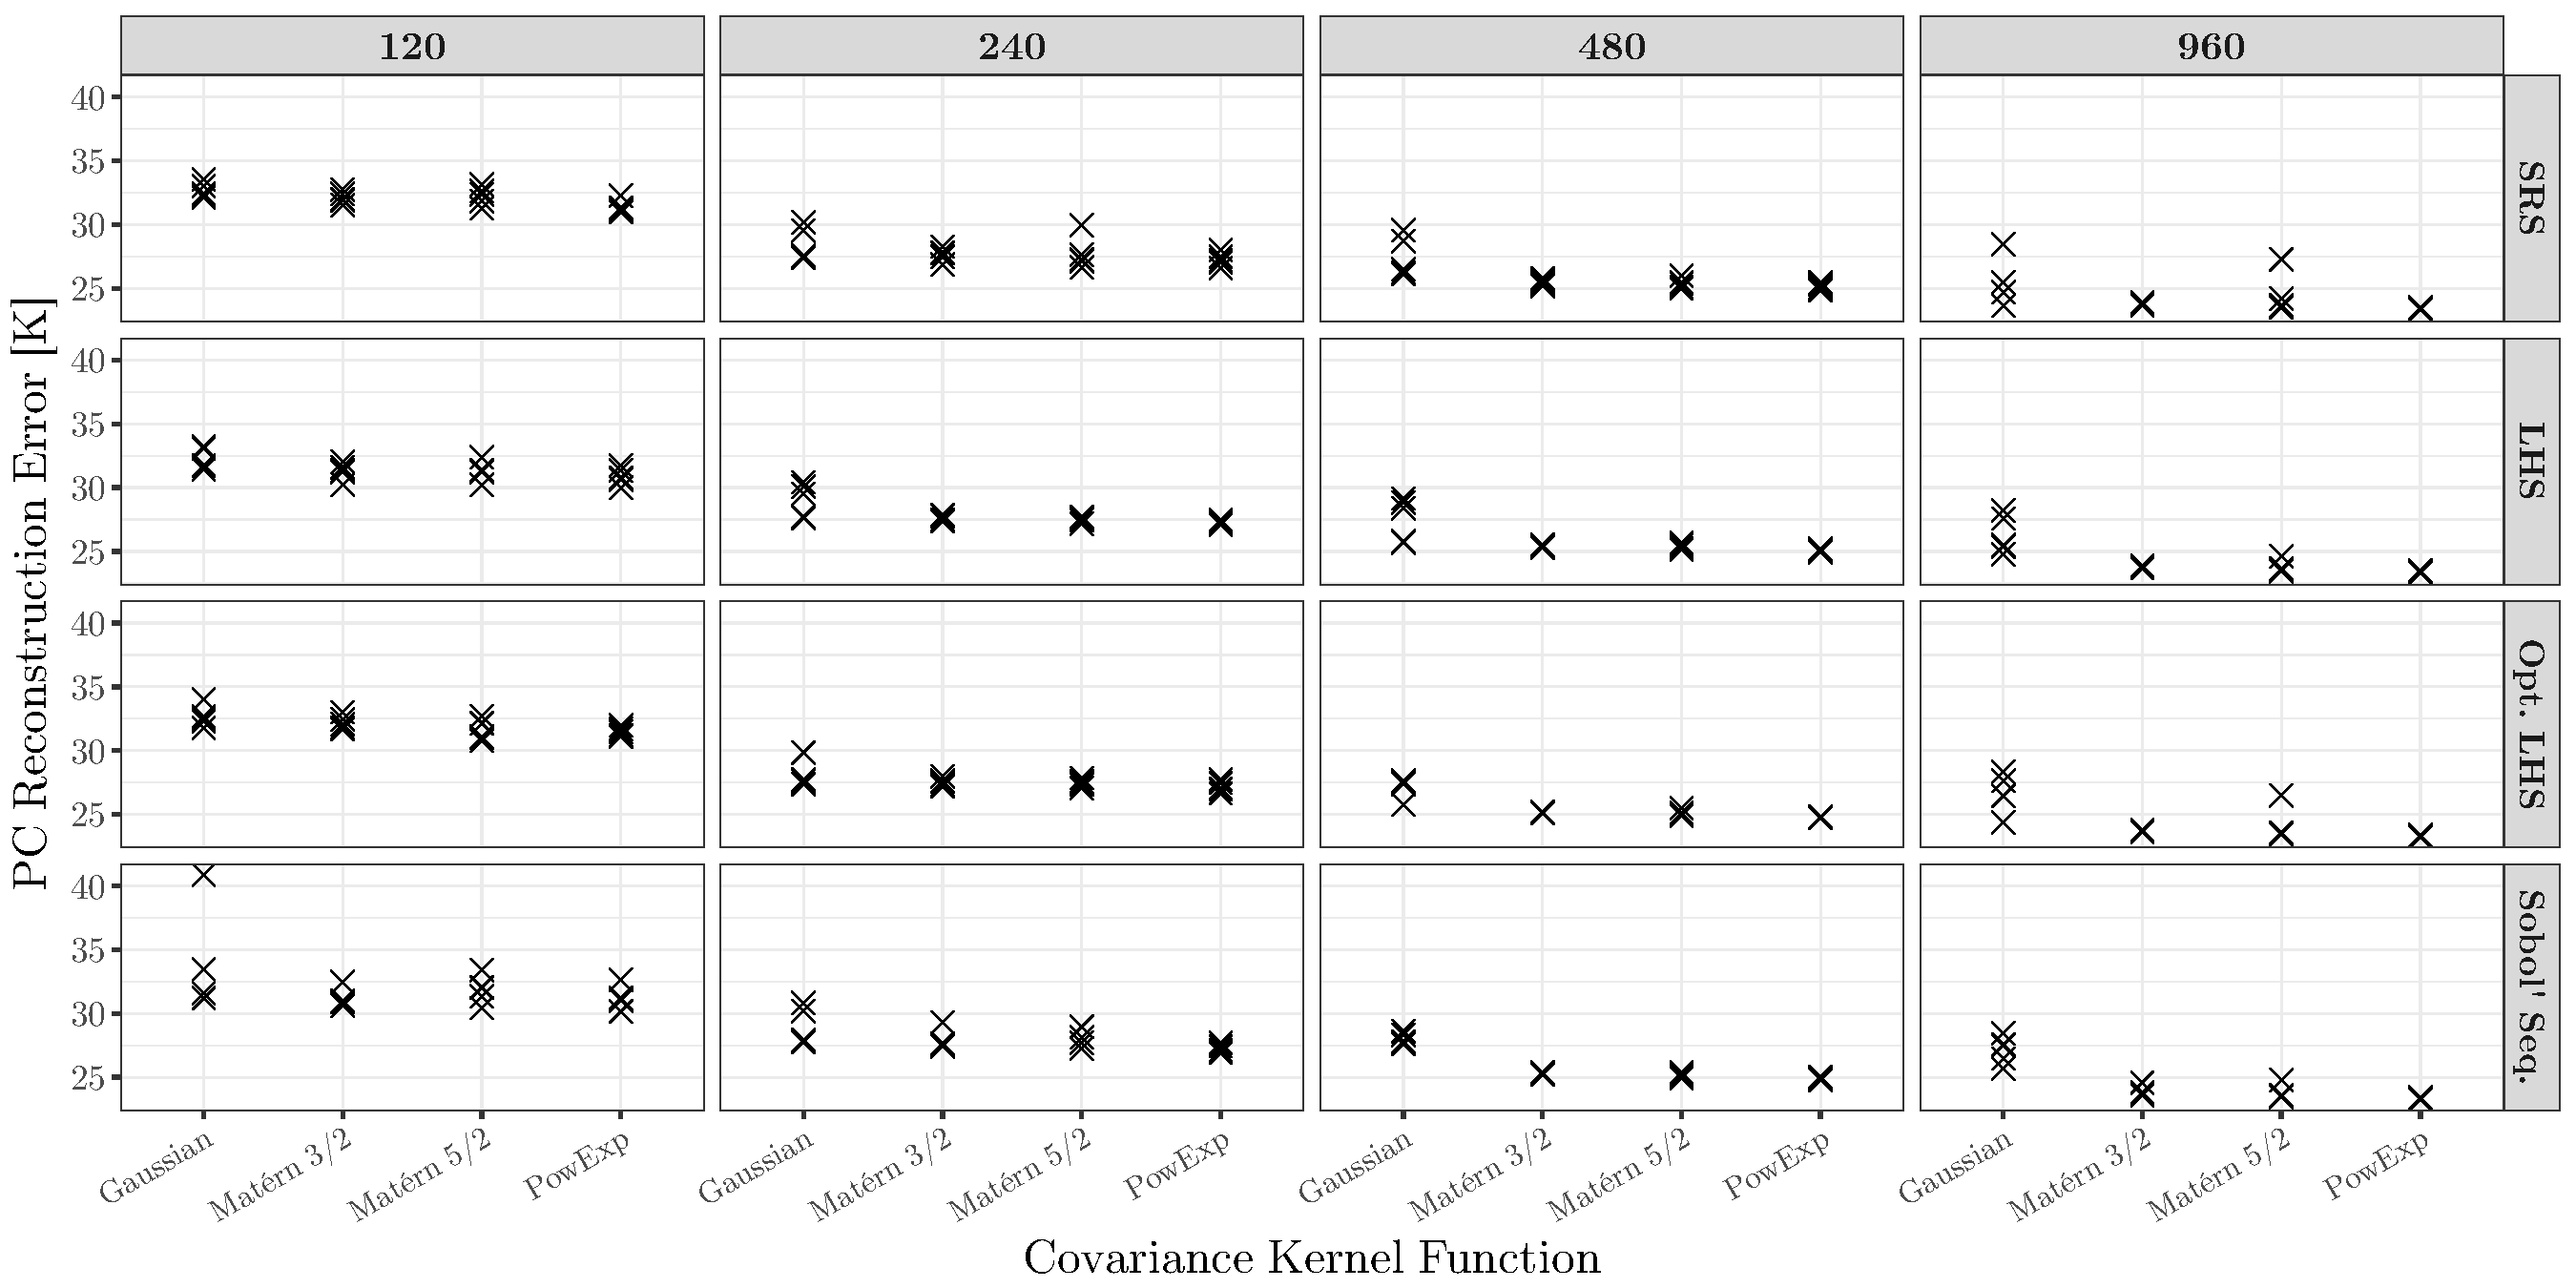
\includegraphics[width=1.0\textwidth]{../figures/chapter4/figures/plotPCGPConstructionTC}
	\caption[The effect of training sample size, experimental design, and covariance function on the predictive performance of GP PC metamodel with respect to the clad temperature output]{The effect of training sample size, experimental design, and covariance function on the predictive performance (in terms of \gls[hyper=false]{rmse}, of \gls[hyper=false]{gp} \gls[hyper=false]{pc} metamodel with respect to the clad temperature output.}
	\label{fig:ch4_plot_pc_gp_construction_tc}
\end{sidewaysfigure}

% Describing the figure itself (as it is the first time it appears)
Fig.~\ref{fig:ch4_plot_pc_gp_construction_tc} summarizes the effect of different training sample sizes, types of experimental design, and types of covariance kernel function on the predictive performance of the constructed \gls[hyper=false]{gp} \gls[hyper=false]{pc} metamodels to predict the clad temperature output.
The training samples were replicated $5$ times for each size and for each design.
The predictive performance was assessed in terms of the \gls[hyper=false]{rmse} which was computed by retaining the first $7$ \gls[hyper=false]{pc} and it was also based on the same validation dataset.
As such the \gls[hyper=false]{rmse} shown in the figure represents the combined error due to \gls[hyper=false]{pc} truncation and misprediction of the standardized \gls[hyper=false]{pc} scores.

% Describing the finding in the figure
It was found that the size of the training sample was the most important factor in determining the predictive performance of a \gls[hyper=false]{gp} \gls[hyper=false]{pc} metamodel.
The choice of covariance function had some effects on the perfomance especially between the smoother covariance functions (i.e., the Gaussian and the Mate\'rn $5/2$) and the less smooth ones (i.e, the power exponential and the Mate\'rn $3/2$).
\gls[hyper=false]{gp} metamodel constructed using the Gaussian covariance kernel function, in particular,
exhibited significant variation in the performance one training sample replication to another compared to the other covariance kernel functions.
Finally, the choice of experimental design for the training sample was found to have a negligible effect on the predictive performance of the \gls[hyper=false]{gp} metamodel.

% The Pressure Drop Output
The \gls[hyper=false]{gp} \gls[hyper=false]{pc} metamodel to predict the pressure drop output also showed the same behavior of being more and more difficult to fit the higher \glspl[hyper=false]{pc} (See Fig.~\ref{fig:ch4_plot_pc_q2_dp}).
\marginpar{\gls[hyper=false]{gp} \gls[hyper=false]{pc} metamodel, pressure drop output}
The \gls[hyper=false]{gp} metamodel for the first standardized \gls[hyper=false]{pc} score remained the easiest to fit.
However, it was also found that the metamodel of the higher \gls[hyper=false]{pc} had a much better convergence property.
That is,
a metamodel with a decent predictive performance could be obtained to predict the standardized \gls[hyper=false]{pc} score as high as the $10$\textsuperscript{th} \gls[hyper=false]{pc} using the considered sample sizes.
\bigfigure[pos=!tbhp,
					 opt={width=0.95\textwidth},
           label={fig:ch4_plot_pc_q2_dp},
           shortcaption={Convergence of \gls[hyper=false]{pc} metamodel with increasing number of training samples with respect to the pressure drop output}]
{../figures/chapter4/figures/plotPCQ2DP}
{Convergence of \gls[hyper=false]{pc} metamodel with increasing number of training samples with respect to the pressure drop output and $Q_2$ validation metric.}

% PC GP Metamodel Construction, Pressure Drop Output
\clearpage
\begin{sidewaysfigure}
	\centering
	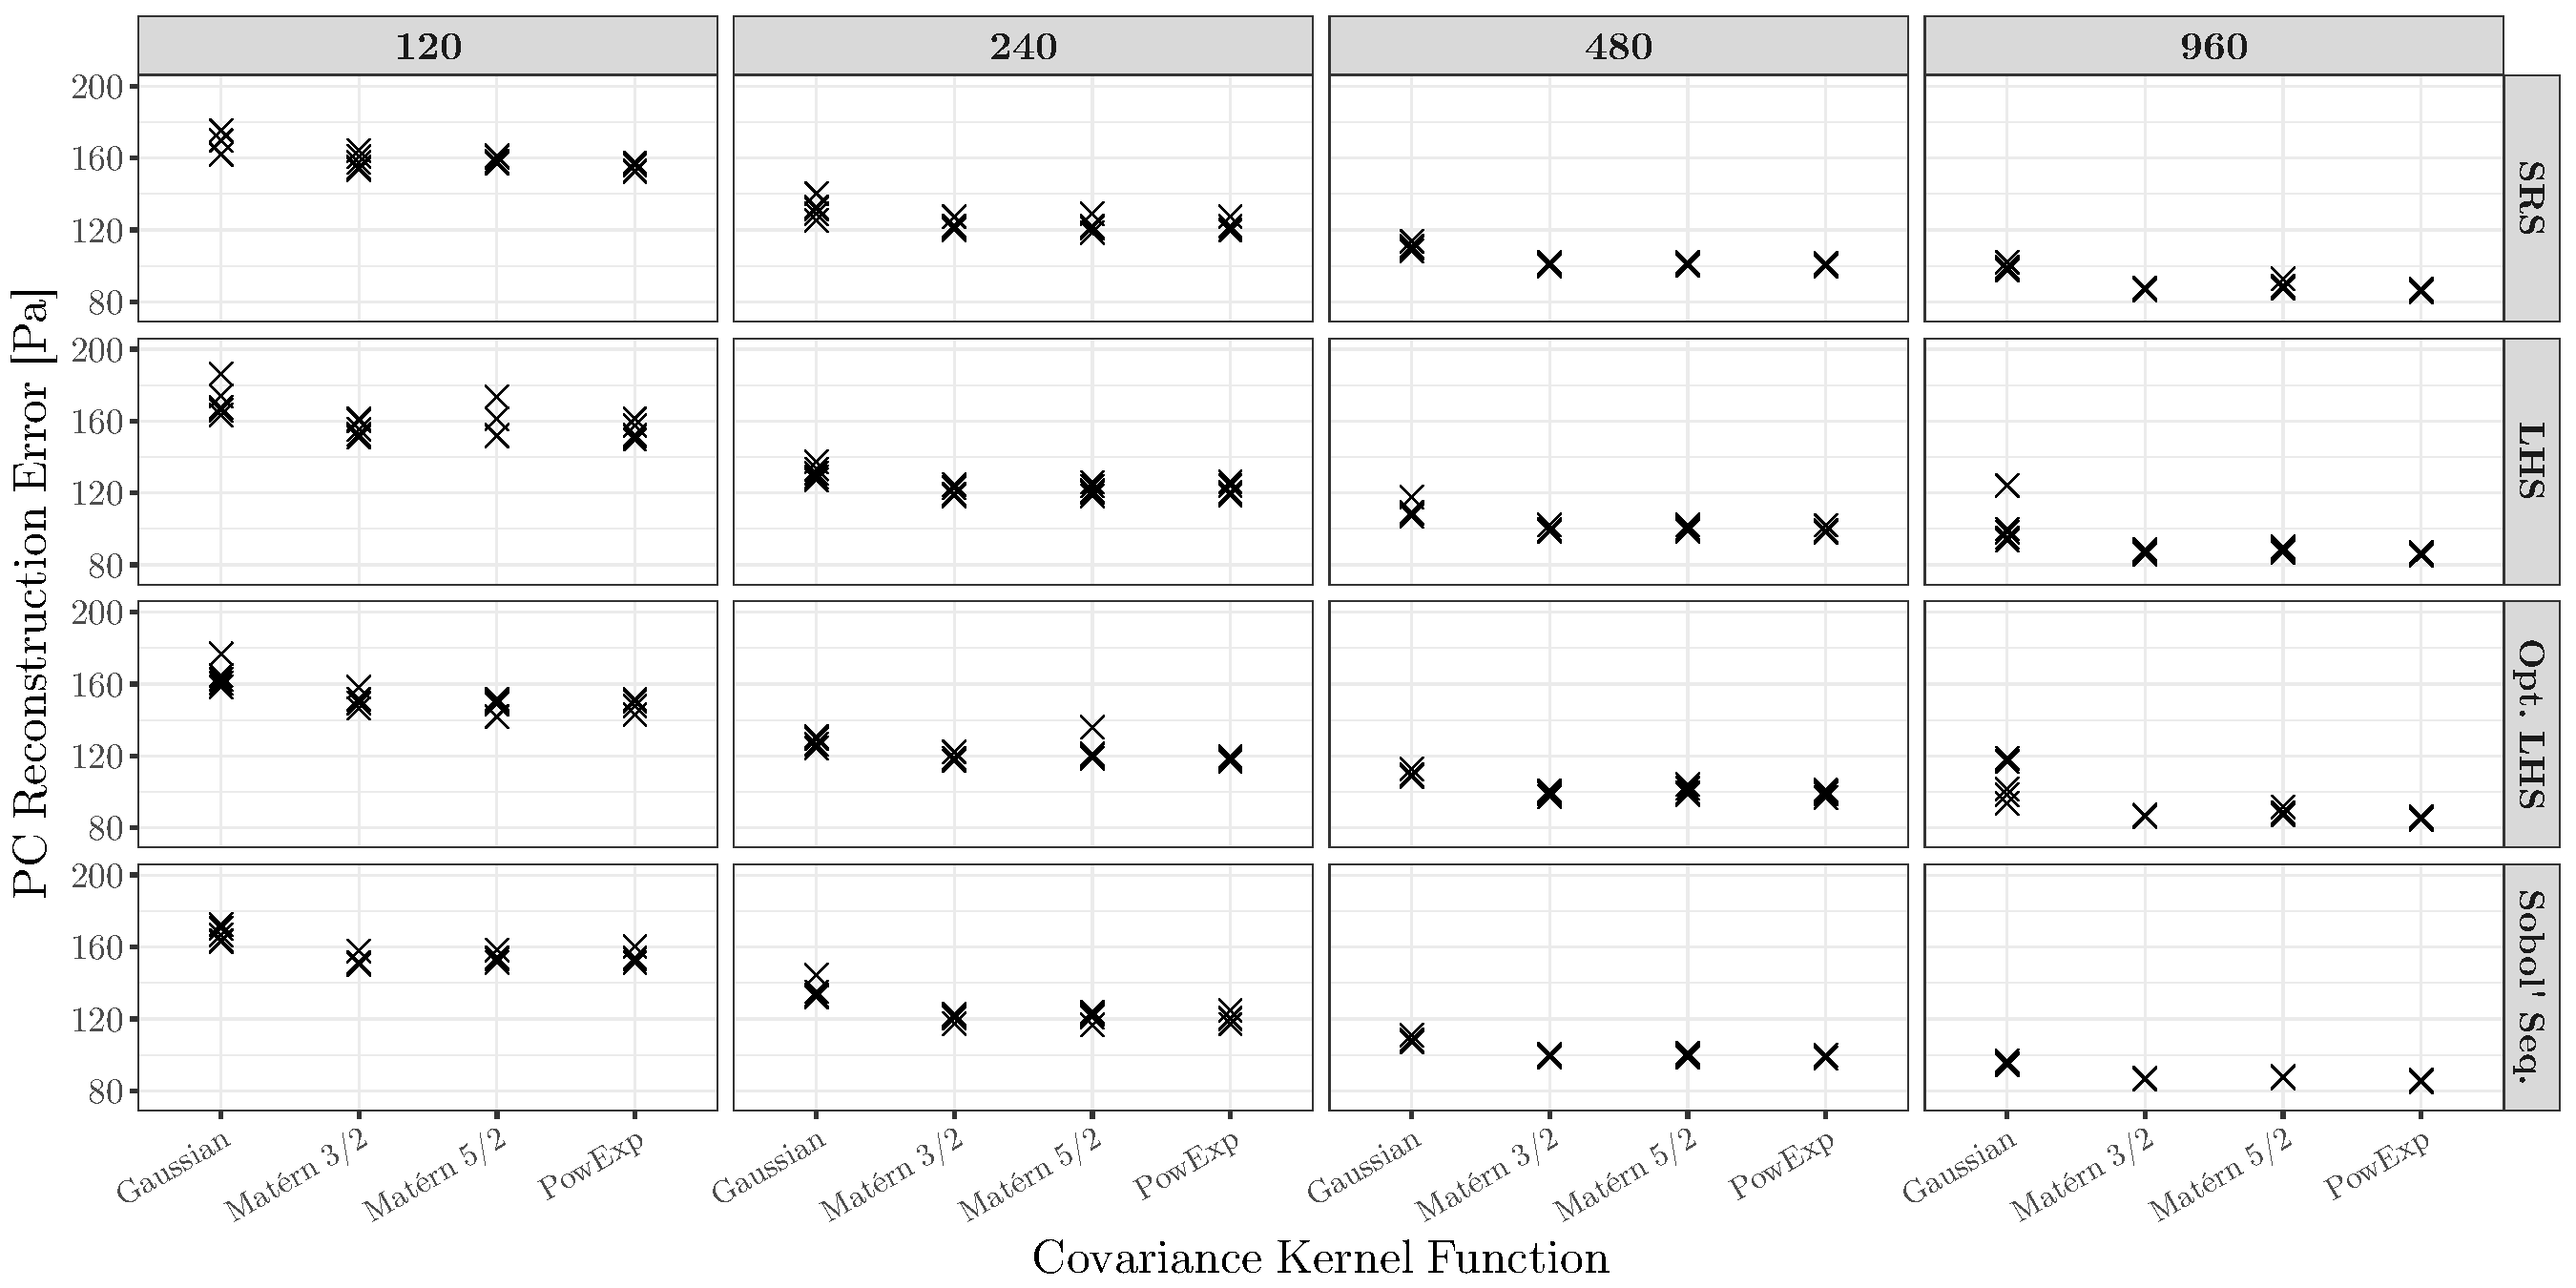
\includegraphics[width=1.0\textwidth]{../figures/chapter4/figures/plotPCGPConstructionDP}
	\caption[The flowchart for the implemented sensitivity analysis methodology applied to the TRACE model of FEBA facility]{The flowchart for the implemented sensitivity analysis methodology applied to the \gls{trace} model of \gls{feba} facility}
	\label{fig:ch4_plot_pc_gp_construction_dp}
\end{sidewaysfigure}
\clearpage

\bigfigure[pos=!tbhp,
					 opt={width=1.0\textwidth},
           label={fig:ch4_plot_pc_q2_co},
           shortcaption={Sobol' Indices estimates with the scores of the warping function for the mid-height clad temperature transient as the \gls[hyper=false]{qoi}}]
{../figures/chapter4/figures/plotPCQ2CO}
{The sensitivity indices with respect to the of the warping function for the mid-height clad temperature transient. Each boxplot represents the bootstrap sample quartile statistics and the vertical line extends the $95$th sample percentile.}


\begin{sidewaysfigure}
	\centering
	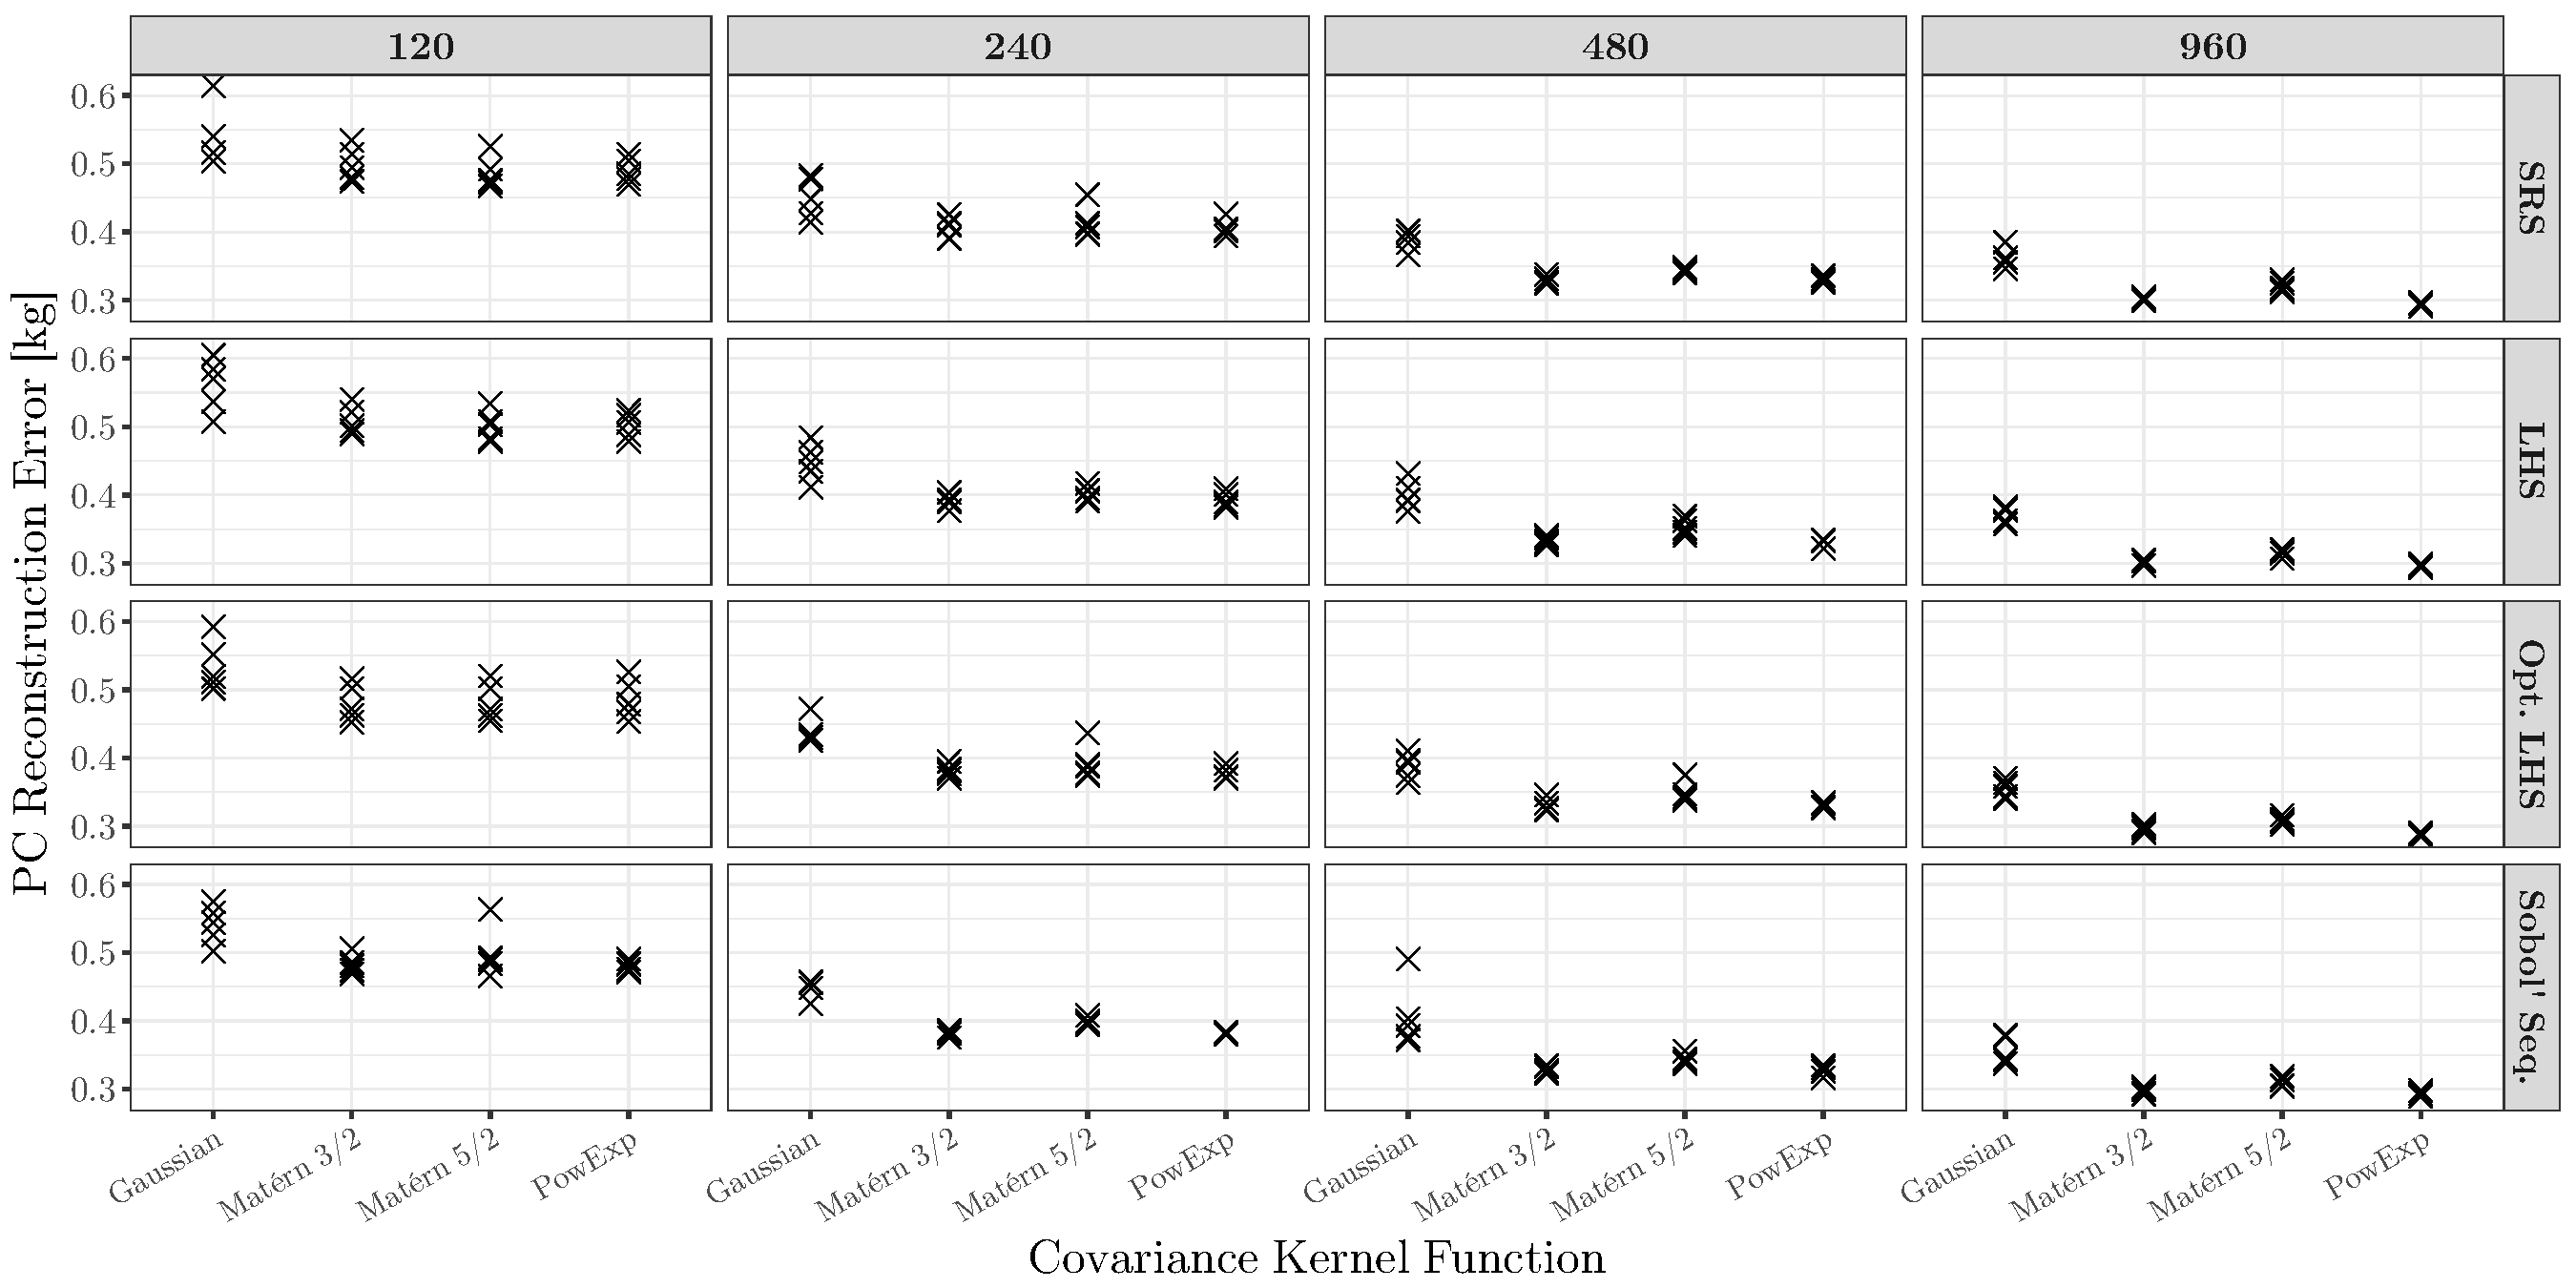
\includegraphics[width=1.0\textwidth]{../figures/chapter4/figures/plotPCGPConstructionCO}
	\caption[The flowchart for the implemented sensitivity analysis methodology applied to the TRACE model of FEBA facility]{The flowchart for the implemented sensitivity analysis methodology applied to the \gls{trace} model of \gls{feba} facility}
	\label{fig:ch4_plot_pc_gp_construction_co}
\end{sidewaysfigure}

\lipsum[20]
